\documentclass{article}
\usepackage{listings}
\usepackage{color}
\usepackage{keyval}
\definecolor{dkgreen}{rgb}{0,0.6,0}
\definecolor{gray}{rgb}{0.5,0.5,0.5}
\definecolor{mauve}{rgb}{0.58,0,0.82}
\usepackage{bookmark}
\usepackage{amsmath}
\usepackage{geometry}
\usepackage{hyperref}
\usepackage{listings}
\usepackage{xcolor}
\usepackage{graphicx}
\usepackage{amsfonts}

\lstset{
  basicstyle=\footnotesize, 
  numbers=left, 
  numberstyle=\tiny\color{gray}, 
  stepnumber=1,
  numbersep=5pt, 
  backgroundcolor=\color{white},
  showspaces=false,
  showstringspaces=false,
  showtabs=false,
  frame=shadowbox,
  rulecolor=\color{black},
  tabsize=2,
  captionpos=b,
  breaklines=true, 
  breakatwhitespace=false, 
  title=\lstname,
  keywordstyle=\color{blue},
  commentstyle=\color{dkgreen},
  escapeinside={\%*}{*)}, 
  morekeywords={*,...} 
}

\begin{document}

To compare the performace of different selection algorithms, I generated arrays in sizes of 100-10000, with a step of 100, and for sequences of each size there will be 25 places uniformly distributed to test the algorithm performance.. The following figure shows the performace of the algorithms for different scales on the size of arrays.

\begin{figure}[htbp]
        \centering
        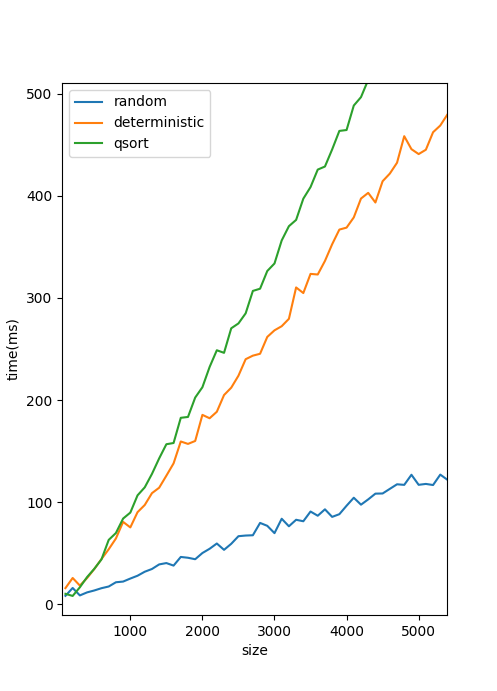
\includegraphics[scale=0.5]{1.png}
\end{figure}

It can be seen that the curve of the random and deterministic selection algoriuthms are all straight lines, which means that the two ar e all of $O(n)$ complexity. The graph of the quick sort algorithm, though not obvious, but it is in fact not a straight line. This phenomenon matches the fact that the algorithm should be of $O(nlogn)$ complexity.

As for the difference between ramdom and dterministic seleciton algorithms, it can be seen that the deterministic selection costs more time than random selection. It is mainly because that the process of recursively finding a pivot is more time-consuming when the size of the sequence is not that large.

So in conclusion, The $O(n)$ random and deterministic selection algorithms have better performance than sorting selection, and random selection works faster than deterministic selection in this size.

The source code are attached in the pages following.

\newpage

{\bf 1. Source Code for algorithms and main function.}
\begin{lstlisting}[title=main.cpp,language=C++]
#include<iostream>
#include "select.h"
using namespace std;

int main(){
    srand(time(NULL));
    int mode,size,k;
    int (*funcs[2])(int *arr,int size,int k) = {rselect,dselect};
    cin >> mode >> size >> k;
    int *arr = new int[size];
    for (int i=0;i<size;i++) cin >> arr[i];
    cout << "The order-" << k << " item is " << funcs[mode](arr,size,k) << endl;
    return 0;
}
    
\end{lstlisting}
\begin{lstlisting}[title=select.h,language=C++]
#ifndef SELECT_H
#define SELECT_H
#include <cstdlib>
#include <algorithm>
#define SWAP(a,b) {if (a!=b) {a = a^b;b = a^b;a = a^b;}}
int rselect(int *arr,int size,int k);
int dselect(int *arr,int size,int k);
void quick_sort_inplace(int *arr,int n);
int sortselect(int *arr,int size,int k);
#endif

\end{lstlisting}
\begin{lstlisting}[title=select.cpp,language=C++]
#include "select.h"

int rselect(int *arr,int size,int k){
    if (size==1) return arr[0];
    if (size==2){
        if (arr[1]<arr[0]) SWAP(arr[1],arr[0]);
        return arr[k];
    }
    int pivot = rand()%size;
    SWAP(arr[pivot],arr[0]);
    int lflag=1,rflag=size-1;
    while (lflag<rflag){
        while ((arr[lflag]<arr[0])&&(lflag<size-1)) lflag++;
        while ((arr[rflag]>=arr[0])&&(rflag>0)) rflag--;
        if (lflag<rflag) SWAP(arr[lflag],arr[rflag]);
    }
    SWAP(arr[0],arr[rflag]);
    if (rflag==k) return arr[rflag];
    if (rflag>k) return rselect(arr,rflag,k);
    return rselect(arr+rflag+1,size-rflag-1,k-rflag-1);
}

int dselect(int *arr,int size,int k){
    if (size<=5) {
        for (int i=0;i<size;i++)
            for (int j=i+1;j<size;j++)
                if (arr[i]>arr[j]) SWAP(arr[i],arr[j]);
        return arr[k];
    }
    int groups = size/5;
    if (size%5==0) groups--;
    int *C = new int[groups];
    for (int i=0;i<groups;i++){
            int nowgroup = i*5;
            for (int j=0;j<3;j++)
                for (int k=j+1;k<5;k++)
                    if (arr[nowgroup+j]>arr[nowgroup+k]) SWAP(arr[nowgroup+j],arr[nowgroup+k])
            C[i] = arr[nowgroup+2];
    }
    int pnum = dselect(C,groups,groups/2);
    delete []C;
    int pivot;
    for (pivot=2;arr[pivot]!=pnum;pivot++);
    SWAP(arr[pivot],arr[0]);
    int lflag=1,rflag=size-1;
    while (lflag<rflag){
        while ((arr[lflag]<arr[0])&&(lflag<size-1)) lflag++;
        while ((arr[rflag]>=arr[0])&&(rflag>0)) rflag--;
        if (lflag<rflag) SWAP(arr[lflag],arr[rflag]);
    }
    SWAP(arr[0],arr[rflag]);
    if (rflag==k) return arr[rflag];
    if (rflag>k) return dselect(arr,rflag,k);
    return dselect(arr+rflag+1,size-rflag-1,k-rflag-1);
}


void quick_sort_inplace(int *arr, int n){
    if ((n==0)||(n==1)) return;
    if (n==2){
        if (arr[0]>arr[1]) SWAP(arr[0],arr[1]);
        return;
    }
    int pivot = rand()%n;
    SWAP(arr[pivot],arr[0]);
    int lflag=1,rflag=n-1;
    while (lflag<rflag){
        while ((arr[lflag]<arr[0])&&(lflag<n-1)) lflag++;
        while ((arr[rflag]>=arr[0])&&(rflag>0)) rflag--;
        if (lflag<rflag) SWAP(arr[lflag],arr[rflag]);
    }
    SWAP(arr[0],arr[rflag]);
    quick_sort_inplace(arr,rflag);
    quick_sort_inplace(arr+rflag+1,n-rflag-1);
}
int cmp(const void *a,const void *b){
    int ta = *((int*)a);
    int tb = *((int*)b);
    return ta-tb;
}
int sortselect(int *arr,int size,int k){
    quick_sort_inplace(arr,size);
    return arr[k];
}
\end{lstlisting}

\end{document}